\documentclass[11pt,a4paper]{article}
\usepackage[utf8]{inputenc}
\usepackage[T1]{fontenc}
\usepackage{lmodern}
\usepackage[margin=0.8in]{geometry}
\usepackage{graphicx}
\usepackage{xcolor}
\usepackage{hyperref}
\usepackage{listings}
\usepackage{booktabs}
\usepackage{enumitem}
\usepackage{fancyhdr}
\usepackage{titlesec}
\usepackage{pagecolor}
\usepackage[most]{tcolorbox}
\usepackage{tikz}
\usetikzlibrary{shapes.geometric, arrows.meta, positioning, calc}

% TikZ styles for flow diagrams
\tikzset{
    process/.style={rectangle, rounded corners, minimum width=2.5cm, minimum height=0.8cm, text centered, draw=border, fill=cardbg, font=\small},
    arrow/.style={thick, ->, >=Stealth, color=textsecondary},
    data/.style={rectangle, minimum width=1.5cm, minimum height=0.6cm, text centered, draw=border, fill=white, font=\small\ttfamily}
}

% Use Helvetica-like font
\usepackage{helvet}
\renewcommand{\familydefault}{\sfdefault}

% Light theme colors
\definecolor{bg}{RGB}{255,255,255}
\definecolor{cardbg}{RGB}{245,245,245}
\definecolor{textprimary}{RGB}{0,0,0}
\definecolor{textsecondary}{RGB}{80,80,80}
\definecolor{textmuted}{RGB}{140,140,140}
\definecolor{border}{RGB}{200,200,200}
\definecolor{accent}{RGB}{60,60,60}

% Hyperref setup
\hypersetup{
    colorlinks=true,
    linkcolor=accent,
    urlcolor=accent,
    pdftitle={S.A.M.S. Documentation},
    pdfauthor={S.A.M.S.}
}

% Header/Footer
\pagestyle{fancy}
\fancyhf{}
\fancyhead[L]{\color{textsecondary}\footnotesize\textsc{S.A.M.S.}}
\fancyhead[R]{\color{textsecondary}\footnotesize\textsc{Documentation}}
\fancyfoot[C]{\color{textmuted}\thepage}
\renewcommand{\headrulewidth}{0pt}

% Section styling
\titleformat{\part}[display]
    {\color{textprimary}\Huge\bfseries\scshape\centering}
    {}
    {0pt}
    {}
    [\vspace{-0.5em}\color{border}\rule{\textwidth}{0.5pt}]

\titleformat{\section}
    {\color{textprimary}\Large\bfseries\scshape}
    {}
    {0em}
    {}
    [\vspace{-0.8em}\color{border}\rule{\textwidth}{0.3pt}]

\titleformat{\subsection}
    {\color{textprimary}\large\bfseries}
    {}
    {0em}
    {}

\titleformat{\subsubsection}
    {\color{textsecondary}\normalsize\bfseries}
    {}
    {0em}
    {}

% Code listing style
\lstset{
    basicstyle=\ttfamily\small\color{textprimary},
    backgroundcolor=\color{cardbg},
    frame=single,
    framerule=0.5pt,
    rulecolor=\color{border},
    breaklines=true,
    columns=fullflexible,
    xleftmargin=1em,
    framexleftmargin=1em,
    aboveskip=1em,
    belowskip=1em
}

% Custom tcolorbox for cards
\tcbset{
    card/.style={
        colback=cardbg,
        colframe=border,
        arc=3pt,
        boxrule=0.5pt,
        left=10pt,
        right=10pt,
        top=8pt,
        bottom=8pt
    }
}

% Custom list styling
\setlist[description]{
    font=\color{accent}\bfseries\ttfamily,
    leftmargin=3cm,
    labelwidth=2.5cm,
    labelsep=0.5cm
}

\setlist[itemize]{
    label=\color{textmuted}\textbullet,
    leftmargin=1.5em
}

\setlist[enumerate]{
    label=\color{textsecondary}\arabic*.,
    leftmargin=1.5em
}

\begin{document}

% Title Page
\begin{titlepage}
    \centering
    \vspace*{2cm}

    \includegraphics[width=0.25\textwidth]{logo.png}\\[1.5cm]

    {\color{textprimary}\fontsize{42}{50}\selectfont\bfseries\scshape S.A.M.S.}\\[0.3cm]
    {\color{textsecondary}\Large Secure Access Management System}\\[3cm]

    \begin{tcolorbox}[card, width=0.7\textwidth, halign=center]
        {\color{textprimary}\large\scshape User Guide \& Security Overview}
    \end{tcolorbox}

    \vfill

    {\color{textmuted}\small Version 1.0}\\[0.3cm]
    {\color{textmuted}\small\today}

    \vspace{1.5cm}

    {\color{border}\rule{0.6\textwidth}{0.3pt}}\\[0.8cm]
    {\color{textsecondary}\footnotesize\ttfamily AES-256-GCM\quad//\quad ARGON2ID\quad//\quad LOCAL ONLY}

\end{titlepage}

% Table of Contents
\tableofcontents
\newpage

% ============================================================================
\part{User Guide}
% ============================================================================

\section{Introduction}

S.A.M.S. (Secure Access Management System) is a \textbf{local-first password manager} designed for security-conscious users. All data is encrypted and stored entirely on your device---no cloud, no servers, no third parties.

\subsection{Key Features}

\begin{tcolorbox}[card]
\begin{itemize}
    \item \textbf{Strong Encryption} --- AES-256-GCM with Argon2id key derivation
    \item \textbf{TOTP Support} --- Built-in two-factor authentication code generation
    \item \textbf{Password Generator} --- Cryptographically secure password creation
    \item \textbf{Expiry Tracking} --- Automatic reminders for credential rotation
    \item \textbf{Offline Operation} --- Works without internet connection
    \item \textbf{Zero Knowledge} --- Your master password never leaves your device
    \item \textbf{File-Based Storage} --- Your data lives in a \texttt{.sams} file you control
\end{itemize}
\end{tcolorbox}

\begin{tcolorbox}[card, colframe=accent]
\textbf{Important:} S.A.M.S. does not auto-save. After making any changes, you must \textbf{save and download} your updated \texttt{.sams} file. Always replace your old file with the new one to avoid data loss.
\end{tcolorbox}

\section{Getting Started}

\subsection{Creating a New Database}

\begin{enumerate}
    \item Launch S.A.M.S. in your web browser
    \item Click \texttt{Initialize New Database}
    \item Enter a strong master password (minimum 8 characters)
    \item Confirm your master password
    \item Click \texttt{Initialize}
\end{enumerate}

\begin{tcolorbox}[card, colframe=accent]
\textbf{Important:} Your master password is the \textit{only} way to access your data. There is no recovery mechanism---if you forget it, your data is permanently inaccessible.
\end{tcolorbox}

\subsection{Opening an Existing Database}

\begin{enumerate}
    \item Click \texttt{Browse} to select your \texttt{.sams} file
    \item Enter your master password
    \item Click \texttt{Decrypt \& Access}
\end{enumerate}

\section{Managing Entries}

\subsection{Adding a New Entry}

The entry form (left sidebar) allows you to store credentials:

\begin{tcolorbox}[card]
\begin{description}
    \item[Title] Required. A name for the entry (e.g., ``GitHub'')
    \item[URL] The website address
    \item[Username] Your login username or email
    \item[Password] Your password (use the generator for secure passwords)
    \item[TOTP Secret] Optional. Base32 secret for 2FA codes
    \item[Docs URL] Link to documentation or admin panel
    \item[Tags] Comma-separated labels for organization
    \item[Notes] Additional information
    \item[Expiry] Password expiration period (or ``Never expire'')
\end{description}
\end{tcolorbox}

\subsection{Using the Password Generator}

\begin{enumerate}
    \item Set desired password length (default: 16 characters)
    \item Select character types:
    \begin{itemize}
        \item \texttt{A-Z} (uppercase letters)
        \item \texttt{a-z} (lowercase letters)
        \item \texttt{0-9} (numbers)
        \item \texttt{!@\#} (symbols)
    \end{itemize}
    \item Click \texttt{Generate}
    \item Preview the password and click \texttt{Use} to apply
\end{enumerate}

\subsection{Setting Up TOTP}

S.A.M.S. can generate 6-digit TOTP codes for your accounts:

\begin{enumerate}
    \item When setting up 2FA on a website, look for the ``setup key'' or ``secret''
    \item Paste it into the TOTP Secret field, or paste the full \texttt{otpauth://} URI
    \item S.A.M.S. will automatically extract and store the secret
    \item TOTP codes appear on entry cards with a countdown timer
\end{enumerate}

\begin{tcolorbox}[card]
\textbf{Tip:} Click on the TOTP code to copy it to your clipboard.
\end{tcolorbox}

\subsection{Editing and Deleting Entries}

\begin{itemize}
    \item Hover over an entry card to reveal action buttons
    \item Click the \textbf{pencil icon} to edit
    \item Click the \textbf{trash icon} to delete (requires confirmation)
\end{itemize}

\section{Search and Organization}

\subsection{Tabs}

\begin{tcolorbox}[card]
\begin{description}
    \item[All] Shows all entries
    \item[Logins] Entries with passwords
    \item[Bookmarks] Entries without passwords (URL-only)
    \item[Expiring] Entries with passwords expiring within 14 days
\end{description}
\end{tcolorbox}

\subsection{Search}

Type in the search box to filter entries by title, URL, username, notes, or tags.

\subsection{Sorting}

Use the sort dropdown to order entries by:
\begin{itemize}
    \item Newest first
    \item Oldest first
    \item Alphabetical (by title)
    \item Expiry date
\end{itemize}

\section{Saving Your Data}

\begin{tcolorbox}[card, colframe=accent]
\textbf{Critical:} S.A.M.S. stores your data in a local \texttt{.sams} file. \textbf{You must save and download the file after every change.} Changes are \textit{not} saved automatically---if you close your browser without saving, your changes will be lost.
\end{tcolorbox}

\subsection{Manual Save}

\begin{itemize}
    \item Click \texttt{Save} in the navigation bar, or
    \item Press \texttt{Ctrl+S} (Windows/Linux) or \texttt{Cmd+S} (Mac)
    \item \textbf{Download the new file} when prompted
    \item Replace your old \texttt{.sams} file with the newly downloaded one
\end{itemize}

An asterisk (*) in the page title indicates unsaved changes.

\subsection{Exporting Data}

\begin{enumerate}
    \item Click \texttt{Export} in the navigation bar
    \item Choose whether to include passwords
    \item Click \texttt{Export CSV} to download
\end{enumerate}

\begin{tcolorbox}[card, colframe=accent]
\textbf{Warning:} CSV exports are unencrypted plain text. Handle with care.
\end{tcolorbox}

\section{Keyboard Shortcuts}

\begin{tcolorbox}[card]
\begin{center}
\begin{tabular}{ll}
\color{accent}\texttt{Ctrl/Cmd + S} & Save database \\
\color{accent}\texttt{Esc} & Close modal dialogs \\
\end{tabular}
\end{center}
\end{tcolorbox}

\newpage

% ============================================================================
\part{Security Overview}
% ============================================================================

\section{Architecture}

S.A.M.S. follows a \textbf{zero-knowledge, local-first} architecture:

\begin{tcolorbox}[card]
\begin{itemize}
    \item All encryption/decryption happens in your browser
    \item No data is transmitted to any server
    \item Your master password never leaves your device
    \item Database files are fully encrypted at rest
\end{itemize}
\end{tcolorbox}

\section{Encryption}

\subsection{Cipher: AES-256-GCM}

S.A.M.S. uses \textbf{AES-256-GCM} (Advanced Encryption Standard with Galois/Counter Mode):

\begin{itemize}
    \item \textbf{256-bit key} --- Provides $2^{256}$ possible keys
    \item \textbf{Authenticated encryption} --- Detects tampering
    \item \textbf{12-byte IV} --- Unique per encryption operation
    \item \textbf{NIST-approved} --- Standard for classified government data
\end{itemize}

\subsection{Key Derivation: Argon2id}

The master password is transformed into an encryption key using \textbf{Argon2id}:

\begin{tcolorbox}[card]
\begin{center}
\begin{tabular}{ll}
\color{textsecondary}Algorithm & \color{textprimary}Argon2id (hybrid) \\
\color{textsecondary}Time Cost & \color{textprimary}3 iterations \\
\color{textsecondary}Memory Cost & \color{textprimary}128 MB \\
\color{textsecondary}Parallelism & \color{textprimary}1 \\
\color{textsecondary}Output Length & \color{textprimary}256 bits (32 bytes) \\
\color{textsecondary}Salt Length & \color{textprimary}128 bits (16 bytes) \\
\end{tabular}
\end{center}
\end{tcolorbox}

\subsubsection{Why Argon2id?}

\begin{itemize}
    \item Winner of the Password Hashing Competition (2015)
    \item Memory-hard: Resistant to GPU/ASIC attacks
    \item Hybrid mode: Combines Argon2i and Argon2d protections
    \item Recommended by OWASP for password storage
\end{itemize}

\subsection{Encryption Process}

\begin{center}
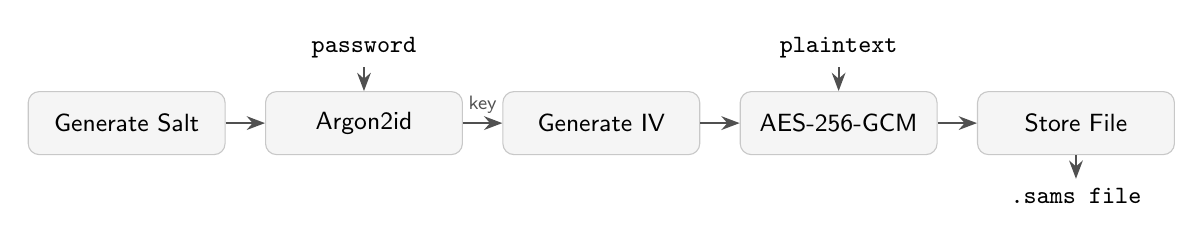
\begin{tikzpicture}[node distance=0.5cm]
    % Nodes
    \node (salt) [process] {Generate Salt};
    \node (derive) [process, right=of salt] {Argon2id};
    \node (iv) [process, right=of derive] {Generate IV};
    \node (encrypt) [process, right=of iv] {AES-256-GCM};
    \node (store) [process, right=of encrypt] {Store File};

    % Input labels
    \node (pwd) [above=0.3cm of derive, font=\small\ttfamily] {password};
    \node (plain) [above=0.3cm of encrypt, font=\small\ttfamily] {plaintext};

    % Output label
    \node (output) [below=0.3cm of store, font=\small\ttfamily] {.sams file};

    % Arrows
    \draw [arrow] (salt) -- (derive);
    \draw [arrow] (derive) -- node[above, font=\scriptsize] {key} (iv);
    \draw [arrow] (iv) -- (encrypt);
    \draw [arrow] (encrypt) -- (store);
    \draw [arrow] (pwd) -- (derive);
    \draw [arrow] (plain) -- (encrypt);
    \draw [arrow] (store) -- (output);
\end{tikzpicture}
\end{center}

\begin{tcolorbox}[card]
\begin{tabular}{ll}
\color{textsecondary}Salt & \color{textprimary}16 random bytes \\
\color{textsecondary}Key & \color{textprimary}256 bits from Argon2id(password, salt) \\
\color{textsecondary}IV & \color{textprimary}12 random bytes \\
\color{textsecondary}Output & \color{textprimary}[salt][IV][ciphertext + auth tag] \\
\end{tabular}
\end{tcolorbox}

\subsection{Decryption Process}

\begin{center}
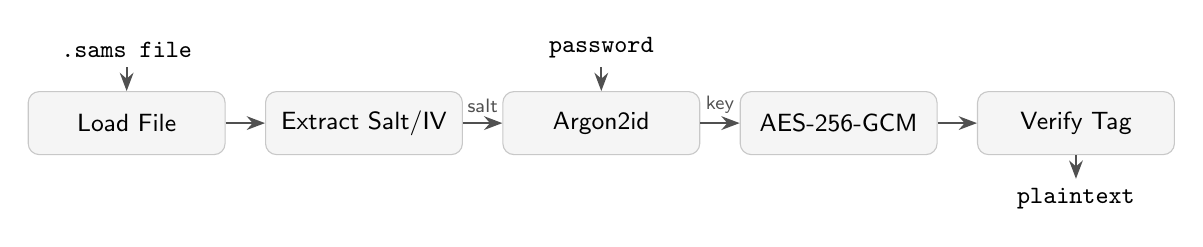
\begin{tikzpicture}[node distance=0.5cm]
    % Nodes
    \node (load) [process] {Load File};
    \node (extract) [process, right=of load] {Extract Salt/IV};
    \node (derive) [process, right=of extract] {Argon2id};
    \node (decrypt) [process, right=of derive] {AES-256-GCM};
    \node (verify) [process, right=of decrypt] {Verify Tag};

    % Input labels
    \node (file) [above=0.3cm of load, font=\small\ttfamily] {.sams file};
    \node (pwd) [above=0.3cm of derive, font=\small\ttfamily] {password};

    % Output label
    \node (output) [below=0.3cm of verify, font=\small\ttfamily] {plaintext};

    % Arrows
    \draw [arrow] (file) -- (load);
    \draw [arrow] (load) -- (extract);
    \draw [arrow] (extract) -- node[above, font=\scriptsize] {salt} (derive);
    \draw [arrow] (derive) -- node[above, font=\scriptsize] {key} (decrypt);
    \draw [arrow] (decrypt) -- (verify);
    \draw [arrow] (pwd) -- (derive);
    \draw [arrow] (verify) -- (output);
\end{tikzpicture}
\end{center}

\begin{tcolorbox}[card]
\begin{tabular}{ll}
\color{textsecondary}Bytes 0--15 & \color{textprimary}Salt \\
\color{textsecondary}Bytes 16--27 & \color{textprimary}IV \\
\color{textsecondary}Bytes 28+ & \color{textprimary}Ciphertext + GCM auth tag \\
\color{textsecondary}Verification & \color{textprimary}Automatic (tampering detected if failed) \\
\end{tabular}
\end{tcolorbox}

\section{TOTP Implementation}

S.A.M.S. implements RFC 6238 (TOTP) and RFC 4226 (HOTP):

\begin{tcolorbox}[card]
\begin{center}
\begin{tabular}{ll}
\color{textsecondary}Algorithm & \color{textprimary}HMAC-SHA1 \\
\color{textsecondary}Code Length & \color{textprimary}6 digits \\
\color{textsecondary}Time Step & \color{textprimary}30 seconds \\
\color{textsecondary}Secret Encoding & \color{textprimary}Base32 \\
\end{tabular}
\end{center}
\end{tcolorbox}

\subsection{Code Generation Algorithm}

\begin{center}
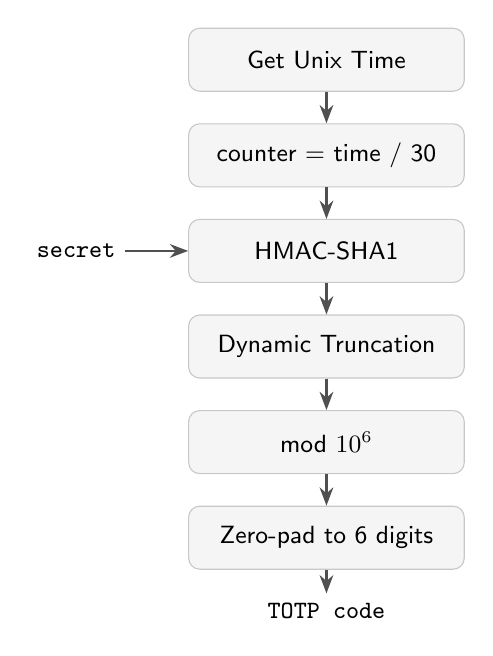
\begin{tikzpicture}[node distance=0.4cm]
    % Nodes - vertical layout for TOTP
    \node (time) [process, minimum width=3.5cm] {Get Unix Time};
    \node (counter) [process, minimum width=3.5cm, below=of time] {counter = time / 30};
    \node (hmac) [process, minimum width=3.5cm, below=of counter] {HMAC-SHA1};
    \node (truncate) [process, minimum width=3.5cm, below=of hmac] {Dynamic Truncation};
    \node (mod) [process, minimum width=3.5cm, below=of truncate] {mod $10^6$};
    \node (pad) [process, minimum width=3.5cm, below=of mod] {Zero-pad to 6 digits};

    % Input
    \node (secret) [left=0.8cm of hmac, font=\small\ttfamily] {secret};

    % Output
    \node (output) [below=0.3cm of pad, font=\small\ttfamily] {TOTP code};

    % Arrows
    \draw [arrow] (time) -- (counter);
    \draw [arrow] (counter) -- (hmac);
    \draw [arrow] (hmac) -- (truncate);
    \draw [arrow] (truncate) -- (mod);
    \draw [arrow] (mod) -- (pad);
    \draw [arrow] (secret) -- (hmac);
    \draw [arrow] (pad) -- (output);
\end{tikzpicture}
\end{center}

\begin{tcolorbox}[card]
\begin{tabular}{ll}
\color{textsecondary}Time Step & \color{textprimary}30 seconds \\
\color{textsecondary}Hash & \color{textprimary}HMAC-SHA1(secret, counter) \\
\color{textsecondary}Truncation & \color{textprimary}Extract 4 bytes at dynamic offset \\
\color{textsecondary}Output & \color{textprimary}6-digit code (000000--999999) \\
\end{tabular}
\end{tcolorbox}

\section{Password Generation}

S.A.M.S. generates passwords using the Web Crypto API:

\begin{lstlisting}
crypto.getRandomValues(Uint32Array)
\end{lstlisting}

This provides \textbf{cryptographically secure pseudo-random numbers} suitable for security-sensitive applications.

\subsection{Password Strength Calculation}

\begin{tcolorbox}[card]
\begin{center}
\begin{tabular}{lc}
\color{textsecondary}Criterion & \color{textprimary}Points \\
\midrule
Length $\geq$ 8 characters & +1 \\
Length $\geq$ 12 characters & +1 \\
Length $\geq$ 16 characters & +1 \\
Contains uppercase \& lowercase & +1 \\
Contains numbers & +1 \\
Contains symbols & +1 \\
\midrule
\textbf{Maximum Score} & \textbf{5} \\
\end{tabular}
\end{center}
\end{tcolorbox}

\section{Data Storage}

\subsection{File Format}

Encrypted databases use the \texttt{.sams} extension:

\begin{lstlisting}
Bytes 0-15:   Salt (16 bytes)
Bytes 16-27:  IV (12 bytes)
Bytes 28+:    Ciphertext + GCM Auth Tag
\end{lstlisting}

\subsection{Entry Structure}

\begin{lstlisting}
{
  id: number,
  title: string,
  url: string,
  username: string,
  password: string,
  totpSecret: string | null,
  tags: string[],
  notes: string,
  docsUrl: string,
  createdAt: ISO date string,
  passwordSetDate: ISO date string,
  expiryDays: number,
  hasPassword: boolean
}
\end{lstlisting}

\section{Security Considerations}

\subsection{Strengths}

\begin{tcolorbox}[card]
\begin{itemize}
    \item \textbf{No network exposure} --- Data never leaves your device
    \item \textbf{Strong encryption} --- AES-256-GCM with authenticated encryption
    \item \textbf{Brute-force resistant} --- Argon2id with 128MB memory cost
    \item \textbf{Unique cryptographic material} --- Random salt and IV per save
    \item \textbf{No backdoors} --- Open architecture with standard algorithms
    \item \textbf{Browser-native crypto} --- Uses Web Crypto API
\end{itemize}
\end{tcolorbox}

\subsection{User Responsibilities}

\begin{itemize}
    \item Choose a strong master password (12+ characters recommended)
    \item Keep your \texttt{.sams} file secure
    \item Maintain regular backups of your database
    \item Use HTTPS when deploying (required for Web Crypto API)
    \item Keep your browser updated
\end{itemize}

\subsection{Threat Model}

\subsubsection{Protected Against}

\begin{itemize}
    \item Remote attacks (no network component)
    \item Database theft (encrypted at rest)
    \item Brute-force attacks (Argon2id memory-hardness)
    \item Data tampering (GCM authentication)
\end{itemize}

\subsubsection{Not Protected Against}

\begin{itemize}
    \item Keyloggers or malware on your device
    \item Weak master passwords
    \item Physical access to unlocked session
    \item Browser vulnerabilities
\end{itemize}

\section{Browser Compatibility}

S.A.M.S. requires Web Crypto API support:

\begin{tcolorbox}[card]
\begin{center}
\begin{tabular}{lc}
\color{textsecondary}Browser & \color{textprimary}Minimum Version \\
\midrule
Google Chrome & 37+ \\
Mozilla Firefox & 34+ \\
Safari & 10.1+ \\
Microsoft Edge & 12+ \\
\end{tabular}
\end{center}
\end{tcolorbox}

\section{Technical References}

\begin{itemize}
    \item NIST SP 800-38D: AES-GCM Specification
    \item RFC 6238: TOTP Algorithm
    \item RFC 4226: HOTP Algorithm
    \item Argon2 Reference: \url{https://github.com/P-H-C/phc-winner-argon2}
    \item Web Crypto API: \url{https://www.w3.org/TR/WebCryptoAPI/}
\end{itemize}

\vfill

\begin{center}
{\color{border}\rule{0.4\textwidth}{0.3pt}}\\[0.8cm]
{\color{textsecondary}\scshape S.A.M.S.}\\[0.2cm]
{\color{textmuted}\small Your credentials, your control.}
\end{center}

\end{document}
